\documentclass{article}

\usepackage{graphicx}
\usepackage{longtable}
\usepackage{subcaption}
\usepackage{caption}
\usepackage{float}
\usepackage{comment}
\graphicspath{{./Images/}}

\begin{document}

\begin{figure}
\centering
	
\includegraphics[height=8cm]{Images/polimi_logo}
\end{figure}
	
\title {{\Huge \it SafeStreets} \\ \Large Software Engineering 2 Project - Prof. Matteo Rossi \\ {\bf DD Document}}
\author{Salvatore Fadda - 944786\\Adriano Mundo - 944684 \\ Francesco Rota - 948714
		\\ \\ A.Y. 2019/2020 \\ Version 1.0}
\date{December 9, 2019}	

\maketitle
\newpage

% Index	
\tableofcontents
\newpage

% Introduction - Section 1
\section{Introduction}
	\subsection{Purpose}
	This document represent the {\it Design Document} (DD). It aims at providing an in-depth description of the architecture below {\it SafeStreets} application and its services. It will present a section related to the architectural design with different perspective on the components of the {\it System}, how they interact and how they will be implemented. All the requirements of the RASD document are mapped with the components to explain how they will be satisfied. Finally, a section for the testing plan for Q\&A team is provided.
		
	\subsection{Scope}
	{\it SafeStreets} is a crowd-sourced application that aims at keeping safe the city's streets. The idea behind this service is to allow {\it Users} to notify the {\it Municipality} when a violation occur on the streets under its jurisdiction. The {\it User} can notice and notify the violation by sending a photo of the violation including date, time and position. {\it SafesStreets} stores all the data and uses a plate recognition algorithm to recognise the image content. \\ \\
	The {\bf Basic Service} allows {\it Users} and {\it Authorities} to mine the information \mbox{collected} by the service, so they can access statistics built from the data. \\ \\
	As {\bf AF1}, the application {\it SafeStreets} identifies potentially unsafe areas and \mbox{suggests} possible interventions to {\it Authorities} to solve the founded issues. \\ \\ 
	As {\bf AF2}. the application {\it SafeStreets} allows the {\it Municipality} to generate \mbox{traffic} tickets directly from the application data. Also, using the data of issued tickets the {\it System} can build statistics and find insights to suggest to {\it Municipality} in order to improve their service.
		
	\subsection{Definitions, Acronyms, Abbreviations}
		\subsubsection{Definitions}
			\begin{itemize}
				\item {\bf Client:} a piece of computer hardware or software that accesses a service made available by a Server. 
				\item {\bf Server:} a computer program or a device that provides functionality and handle the requests of other programs or devices, called Clients. 
				\item {\bf N-Tier:} or multilayer is an architecture in which presentation, application processing, and data management functions are physically separated in n-layers. 
				%%\item {\bf Design Pattern:}
				%%\item {\bf Proxy:}
			\end{itemize}
	
	
		\subsubsection{Acronyms}
			\begin{itemize}
				\item {\bf GPS:} Global Positioning System
				\item {\bf API:} Application Programming Interface
				\item {\bf RASD:} Requirements Analysis and Specification Document
				\item {\bf DBMS:} Data Bases Management System
				\item {\bf GDPR:} General Data Protection Regulation
				\item {\bf MVC:} Model-View-Controller
				\item {\bf REST:} REpresentational State Transfer
				\item {\bf Q\&A:} Quality and Assurance
				\item {\bf UI:} User Interface
				\item {\bf HTTPS:} Hyper Text Transfer Protocol Secure
			\end{itemize}
		
		\subsubsection{Abbreviations}
			\begin{itemize}
				\item {\bf [Rn]:} n-th Functional Requirement
				\item {\bf A1:} Advanced Function One
				\item {\bf A2:} Advanced Function Two 
			\end{itemize}
	
	
		\subsection{Revision history}
			\begin{table}[ht]
				\centering
				\begin{tabular}{ccc} 
				Version & Date & Description  \\ 
				\hline
		 		\\1.0 & 09/12/2019 & First Delivery
		 		\\
			\end{tabular}
			\caption{Revision History}
			\label{default}
		\end{table}
	
	
		\subsection{Reference Documents}
			\begin{itemize}
				\item Mandatory Project Assignment
				\item RASD Document of {\it SafeStreets} application
			\end{itemize} 
	
		\subsection{Document Structure}
		The other sections of the Design Document (DD) are organised in this way:
			\begin{itemize}
				\item {\bf Architectural Design} (Section 2): an in-depth description of the System's architecture. It defines the main components, the relationship between them and the deployment of components. There are different views and levels of analysis of the components plus some subsection useful for identifying how the components interact and the architectural styles and patterns. 
				\item {\bf User Interface Design} (Section 3): a complementary section of what was included in the RASD. It includes the definition of the UX process through a model that represents the flows of the interfaces. 
				\item {\bf Requirements Traceability} (Section 4): a complementary section of what was included in the RASD. It contains all the identified requirements and show the relationship between them and design choices in order to satisfy them. 
				\item {\bf Implementation, Integration and Test Plan} (Section 5): shows the order of the implementation and integration of all the components and subcomponents, providing how the application will be tested.
				\item {\bf Effort Spent} (Section 6): a section containing a table for identifying the hours and the effort spent by each team member to deliver the DD.
			\end{itemize}
		
		\pagebreak
	
	
% Architectural Design - Section 2
\section{Architectural Design}

	\subsection{Overview}
		\begin{figure}[H]
			\centering
			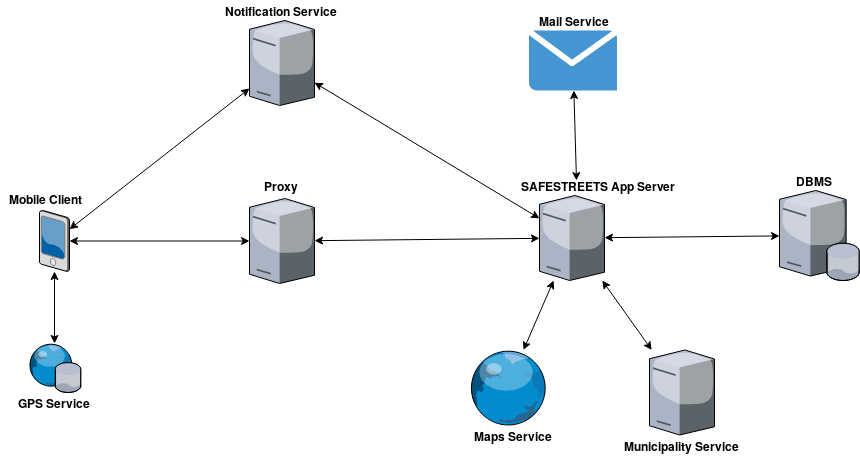
\includegraphics[scale=0.35]{Images/Diagrams/overview_diagram.png}
			\caption{Overview of the System}
		\end{figure}
	The image above shows an high-level overview of the {\it System}'s architecture.
	The components interact with some external services. \\
	The Mobile Client application accesses the GPS service in order to retrive geographical information and communicates with the Application Server through a Proxy. \\ The Application Server uses an external Notification Service to send notifications directly to the Client. It uses a Mail System service and a Map service to execute all the functions. Finally, it accesses the Municipality Service to retrieve data and to communicate with the Municipality through the an API service offered by the Municipality itself.\\ 
	Further details on the {\it System} components will be explained in the next sections. 		
	\pagebreak	
	
	\subsection{Component View}
		\begin{figure}[H]
			\centering
			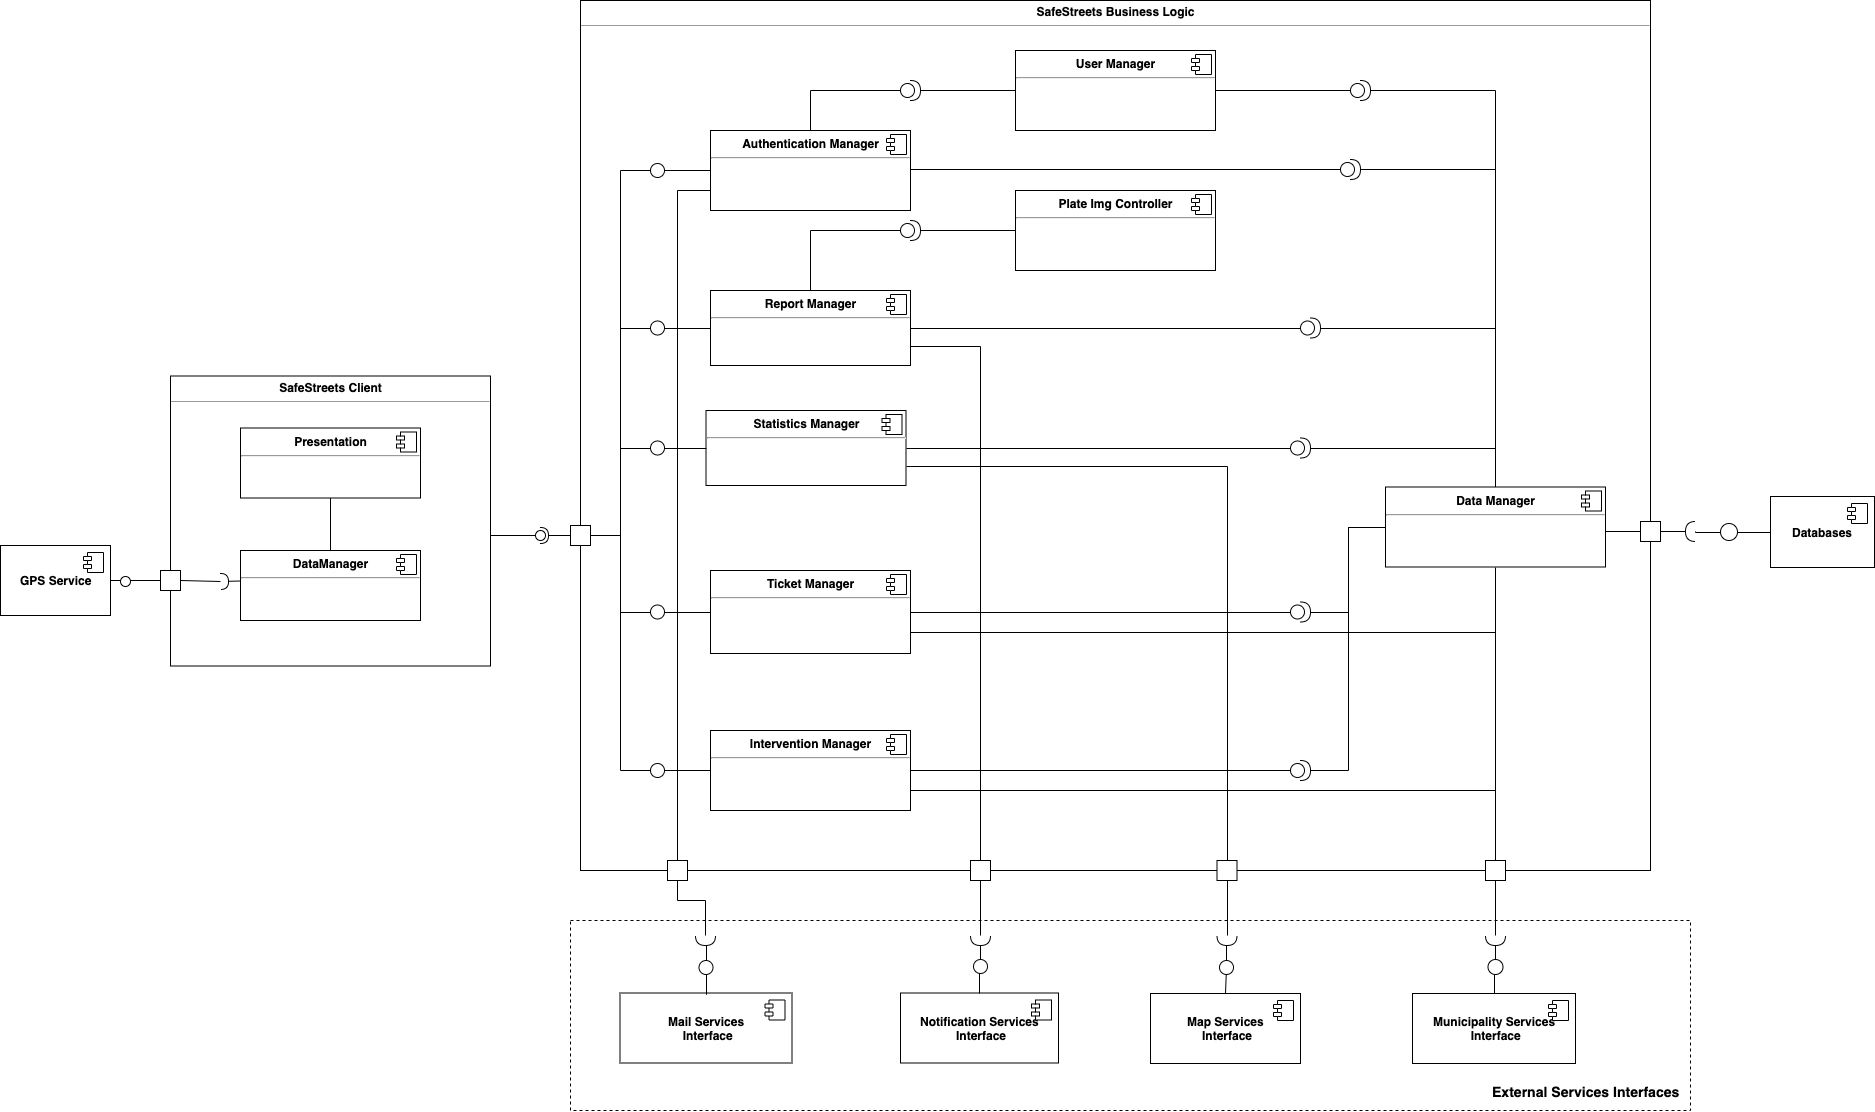
\includegraphics[scale=0.20]{Images/Diagrams/component_diagram.png}
			\caption{{\it SafeStreets} Component Diagram}
		\end{figure}
		The purpose of the UML component diagram is to capture the internal architecture of the {\it System}, showing the structure pf components, how they are connected together as a part of larger components. \\
		It's divided in three main components: the {\it SafeStreets} Client Application, the Business Logic and the external Database. \\ 
		Each main component is divided in modular components to provide specific functionalities. Components communicate between each other by providing interfaces with the required information. \\
		This diagram uses assembly connectors for internal interfaces and delegation connectors for external interfaces. 
		\\ \\
		{\bf SafeStreets Client} \\
		This component located on the {\it User}'s device represents the client machines that access to the Business Logic container. Its sub-modules are the Presentation and Data Manager. It is implemented as a thin-client, so does not contain any logic of the {\it System}.
		\begin{itemize}
		\item {\bf Presentation:} this module corresponds to the View of the MVC Pattern, requires data from the Business Logic to display the correct UI to the {\it User}.
		\item {\bf Data Manager:} this module has to communicate with the GPS Service in order to retrieve the data required to the application. 
		\end{itemize} 
		{\bf SafeStreets Business Logic} \\
		This component contains all the {\it SafeStreets} application logic. It's a module between the Client Application and the Database. It collects together all the components needed to satisfy the application functionalities. In the section below each component will be described.
		\begin{itemize}
		\item {\bf Authentication Manager:} this component contains all the methods needed to access the application, so for the purpose of the system authentication. It's responsible for both the registrazione and log-in process. It continuously interacts with the Database through the Data Manager interface. It guarantees that all the constraints are respected and finally, when you need to confirm to the {\it Users} they have successfully registered, it communicates with the Mail Service Interface to send the confirmation e-mail. 
		\item {\bf User Manager:} this component handles all the functionalities related to the User account, both for simple {\it Users} and {\it Authorities}. Its services are performed by interacting with the Database through the Data Manager. 
		\item {\bf Report Manager:} this component contains the logic needed to perform and handle the violation reported by the {\it User}. Its service are linked to the image loading, the violation indication type and so on. It interacts with another component that's responsible for analysing the image, the Plate Img Controller and stores all the data in the Database through the Data Manager.  Finally, the Report Manager communicates with the Notification Service Interface because it gives a direct feedback to the {\it User} about the loaded image through a push notification.
		\item {\bf Plate Img Controller:} this component handles the request coming from the {\it User} that wants to load a violation image. The request comes from the Report Manager, in fact the component exposes the methods to verify that the image was not modified by third parties, so it makes a consistency check. In order to do this task, the component runs an algorithm.
		\item {\bf Statistics Manager:} this component manage and calculate all the statistics that the application is intended to provide to both {\it Users} and {\it Authorities}. It has two main task: retrieve and store the data from the Database through the Data Manager, where are stored all the data inserted from the application's users; and to calculate all the statistics that are accessible from the UI. It manipulates all the data in order to show simple graphs or to find useful insights. It accesses to Map Services Interface because it needs to retrieve geographical information in order to show statistics directly associated with the city's zone.
		\item {\bf Ticket Manager:} this component is responsible for the ticket verification by the {\it Authorities} thanks to reported {\it User} violation data. In fact he retrieve from the Database through the Data Manager all the violation reported from the {\it Users}, then let the verification to be done manually by an {\it Authorities}, exposing all the needed functions. Finally, it communicates with the Municipality Service Interface in order to advise that the ticket is verified. Therefore the Municipality is able to generate a ticket from this information.
		\item {\bf Intervention Manager:} this component handles the information coming from the Municipality, in fact it interacts with the Municipality Service Interface to retrieve data about accidents. Then, it cross the information with the data stored in the Databases and retrieved through the Data Manager in order to provide suggestions on interventions. 
		\item {\bf Data Manager:} this component provides all the methods to interact with the Database such as data retrieval, storage and update, it is the unique point of access to the Database. 
		\end{itemize}
		{\bf Data Base} \\
		This component represents the DBMS, which provides the interfaces to retrieve and store the data. Data about the application and data about Users are securely stored and encrypted.
		\\ \\
		{\bf External Services Interfaces} \\
		Some components of the diagrams that represent the {\it SafeStreets System} and described above communicate with external components. This are are third party services that expose their API. These communications are bilateral and essential to guarantee all the functionalities. 
		\begin{itemize}
			\item {\bf GPS Service:} this interface communicates with the Client Application that have to access data from the {\it User}'s device, in particular GPS data through the Data Manager interface. GPS data are essential for tracking position and retrieve all suitable metadata necessary to the application to work properly. 
			\item {\bf Mail Services Interface:} this interface is responsible for the interaction with the {\it User} when it's sent a confirmation e-mail after the registration phase. It's accessed by the Authentication Manager.
			\item {\bf Notification Services Interface:} this interface is needed to send push-notification to the {\it User} as an alert when the image processing is not done correctly, so it needs to communicate with the Report Manager in order to advise the {\it User} that have to re-do the process of reporting. 
			\item {\bf Map Services Interface:} this interface is essential for {\it SafeStreets}, in fact access to a mapping service is necessary to show and calculate statistics with respect to the different city's zone. It's a service accessed by the Statistics Manager.
			\item {\bf Municipality Services Interface:} this interface is essential to have a means of communication with the Municipality services. It lets to retrieve data and to pass information to the Municipality in order to do all the services offered by the {\it System}. It's accessed by Ticket, Intervention Mngs. 
		\end{itemize}
		
		\pagebreak
		
	\subsection{Deployment View}
		\begin{figure}[H]
			\centering
			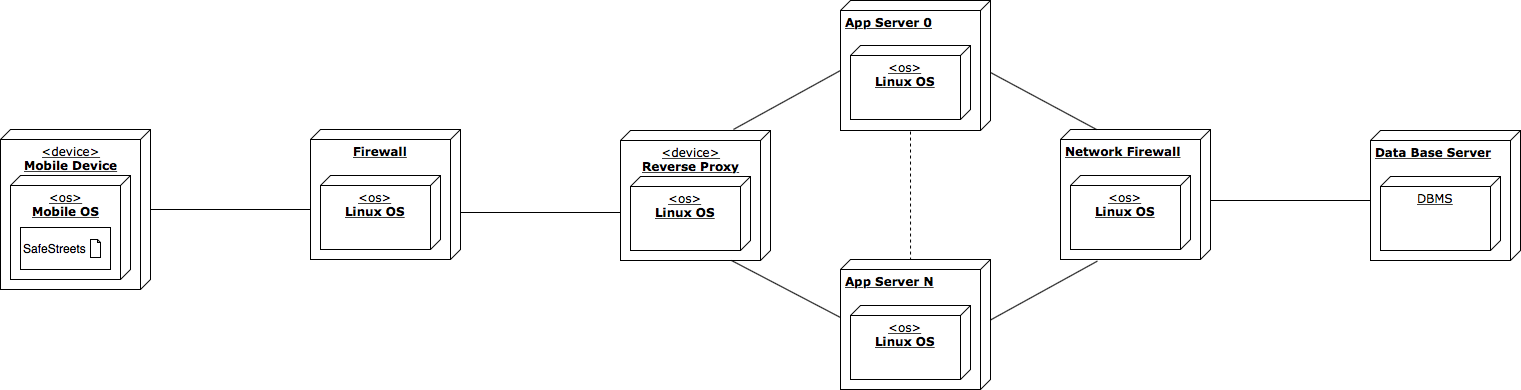
\includegraphics[scale=0.25]{Images/Diagrams/deployment_diagram.png}
			\caption{{\it SafeStreets} Deployment Diagram}
		\end{figure}
		
	The {\it System} presents a Multi-tier architecture. The role of each node will be specified in the next section. \\ \\
			{\bf Mobile Device} \\
			It represents the Client in the architecture, hosting the System’s mobile application. This is equally valid for both Users and Authorities. \\ \\
			{\bf Firewall}\\
			It filters the access to the Reverse Proxy and is used to protect a trusted network from an untrusted network. A firewall provides protection from unauthorized requests or from malicious attacks. \\ \\
			{\bf Reverse Proxy}\\
			It retrieves resources on behalf of a client from the servers and balances the load of the various requests. It helps to achieve increased parallelism and scalability of the application. \\ \\
			{\bf Application Servers}\\
			They include all the business logic of the system, which is completely replicated to allow workload balancing. \\ \\
			{\bf Network Firewall}\\
			It does the same job of the Proxy Firewall but protecting and filtering the access to the DBMS. \\ \\
			{\bf Data Base Server}\\
			All data are stored in the Data Base Server equipped with a relational DBMS and can be retrieved with appropriate queries. \\ \\
	

	\subsection{Runtime View}
	
	{\bf Account Creation Runtime View} \\
	The first sequence diagram \\
	\begin{figure}[H]
			\centering
			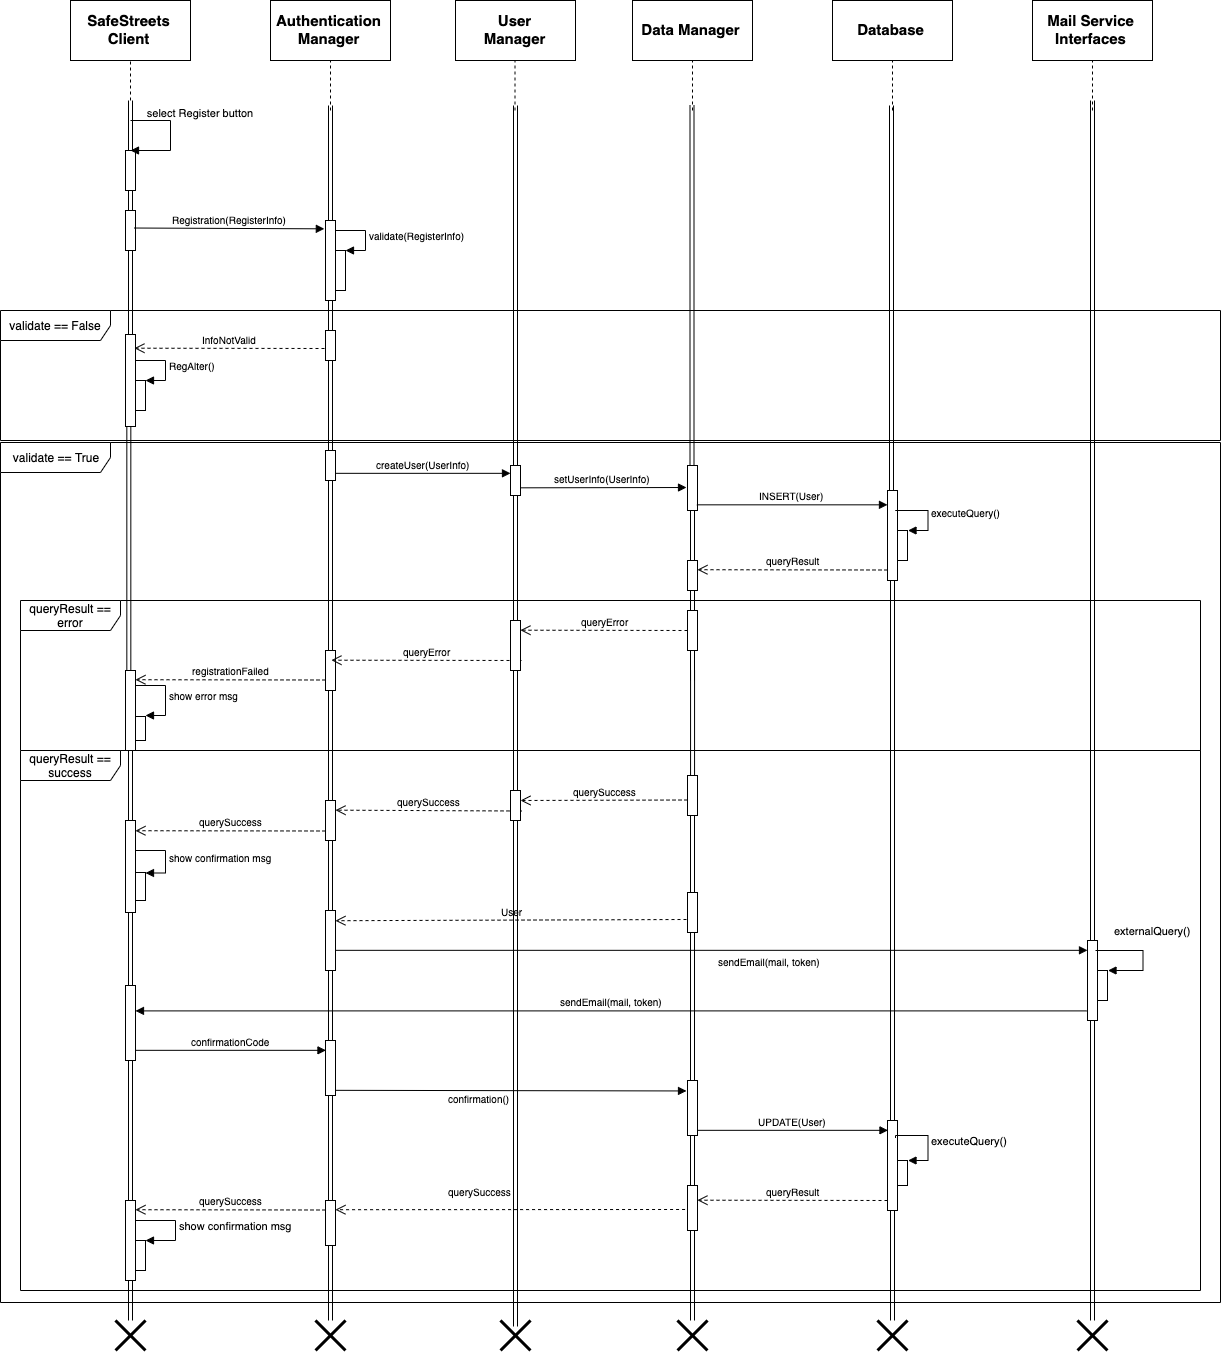
\includegraphics[scale=0.25]{Images/Diagrams/Runtime/registration_runtime.png}
			\caption{{\it SafeStreets} Account Creation Runtime View}
	\end{figure}	
	\pagebreak
	\noindent
	{\bf Log-in Runtime View} \\
	The second sequence diagram \\
	\begin{figure}[H]
			\centering
			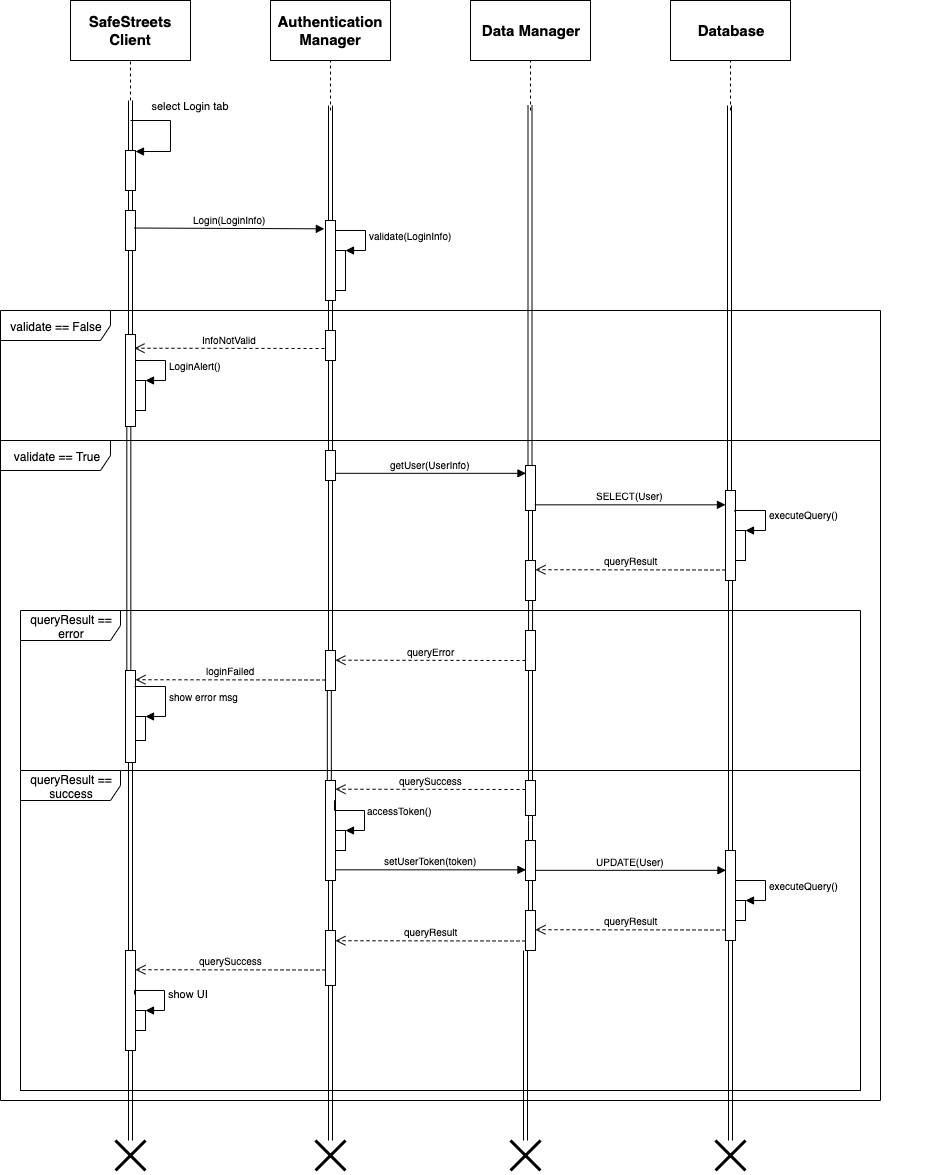
\includegraphics[scale=0.35]{Images/Diagrams/Runtime/login_runtime.png}
			\caption{{\it SafeStreets} Login Runtime View}
	\end{figure}
	\pagebreak
	\noindent	
	{\bf Report Violation Runtime View} \\
	The third sequence diagram \\
	\begin{figure}[H]
			\centering
			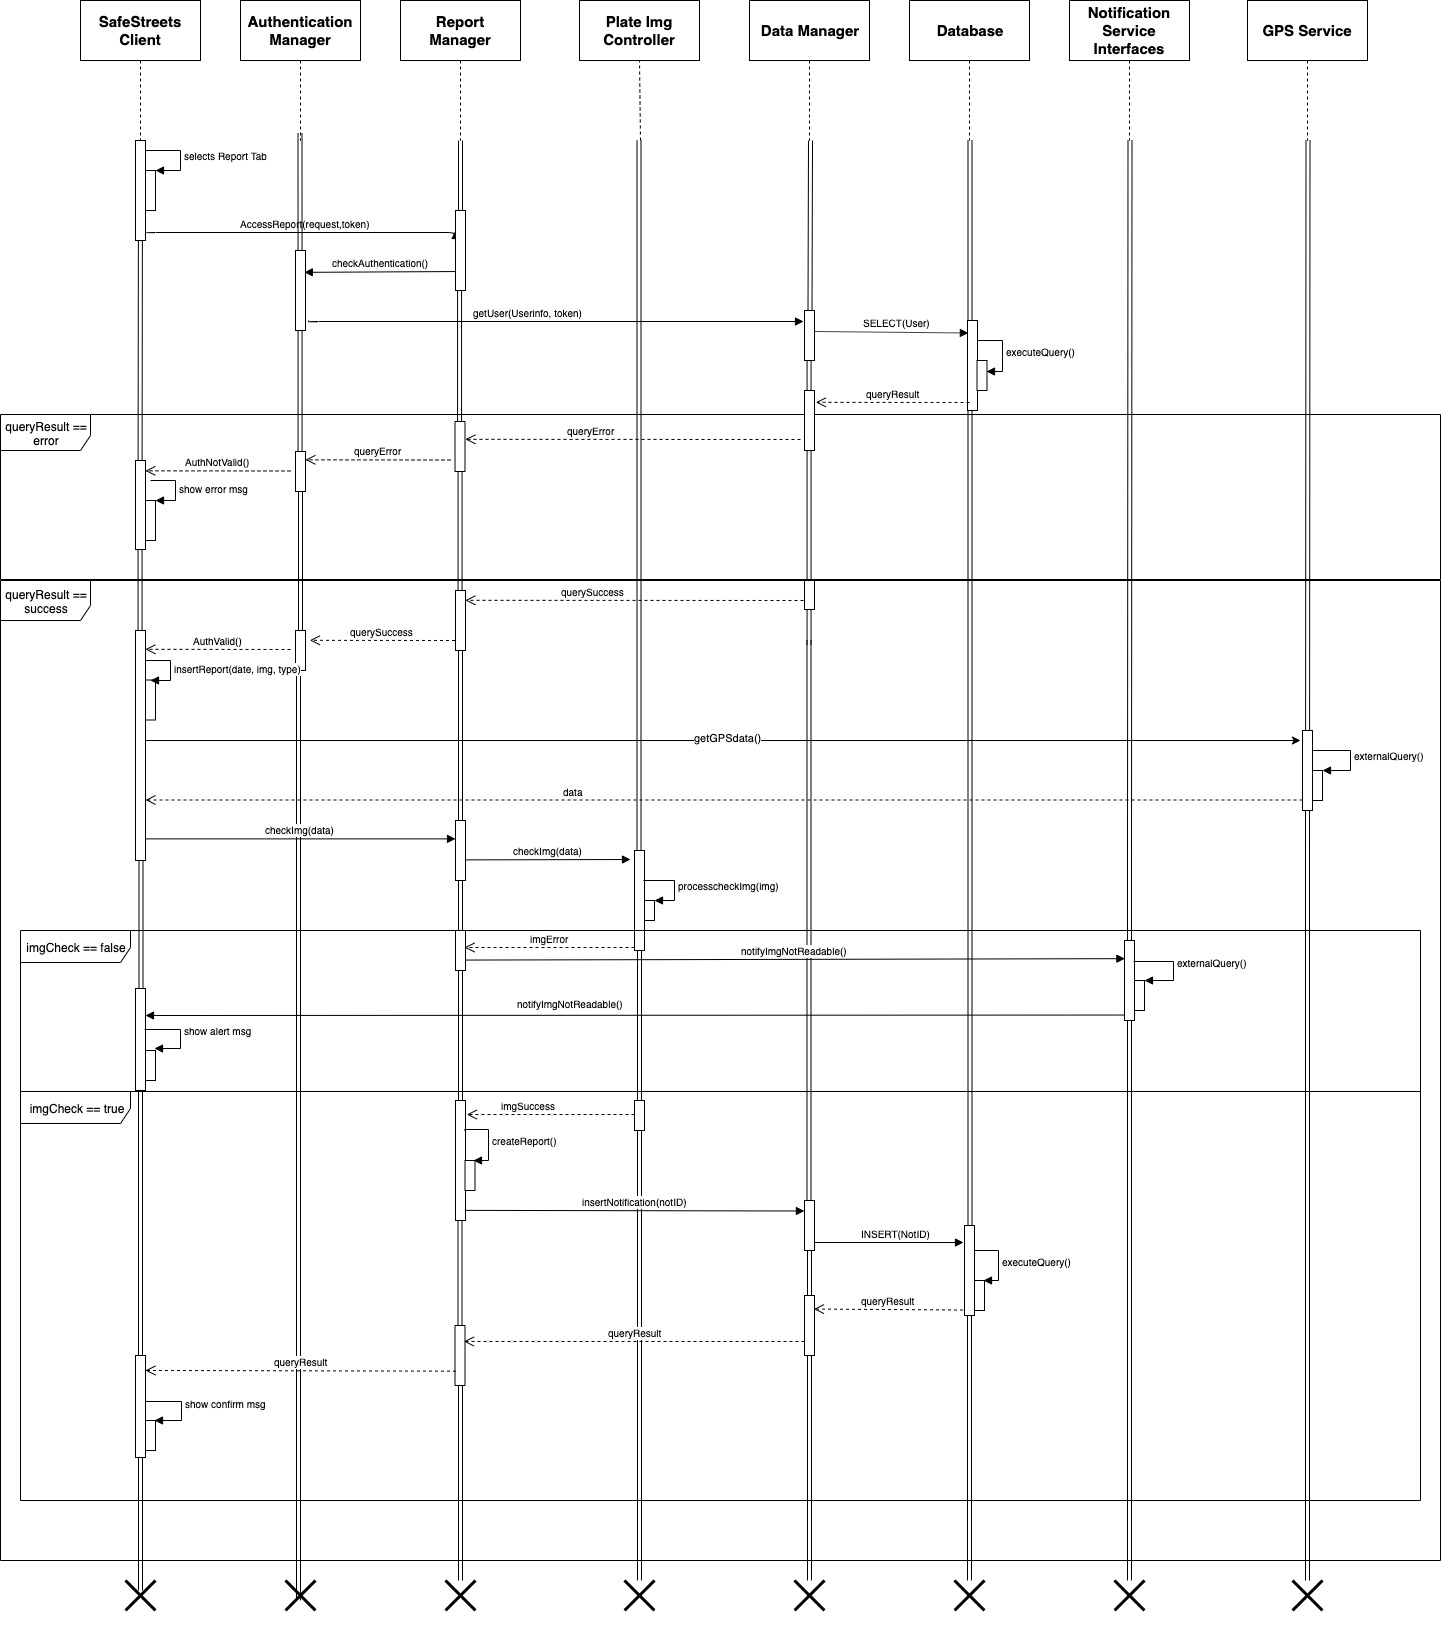
\includegraphics[scale=0.25]{Images/Diagrams/Runtime/report_runtime.png}
			\caption{{\it SafeStreets} Report Violation Runtime View}
	\end{figure}
	\pagebreak
	\noindent
	{\bf Maps Access Runtime View} \\
	The fourth sequence diagram \\
	\begin{figure}[H]
			\centering
			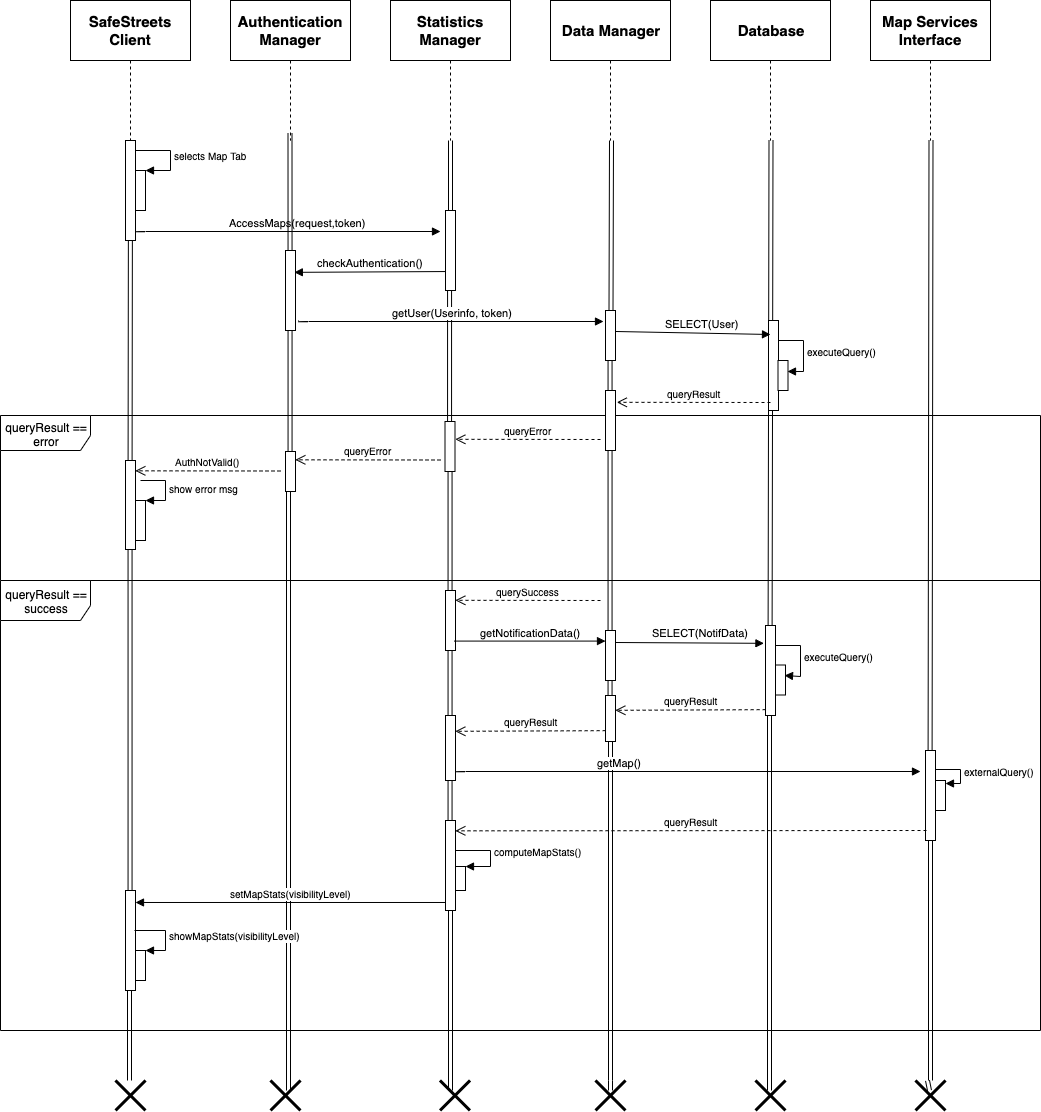
\includegraphics[scale=0.25]{Images/Diagrams/Runtime/maps_runtime.png}
			\caption{{\it SafeStreets} Maps Access Runtime View}
	\end{figure}
	\pagebreak
	\noindent
	{\bf Statistics Access Runtime View} \\
	The fifth sequence diagram \\
	\begin{figure}[H]
			\centering
			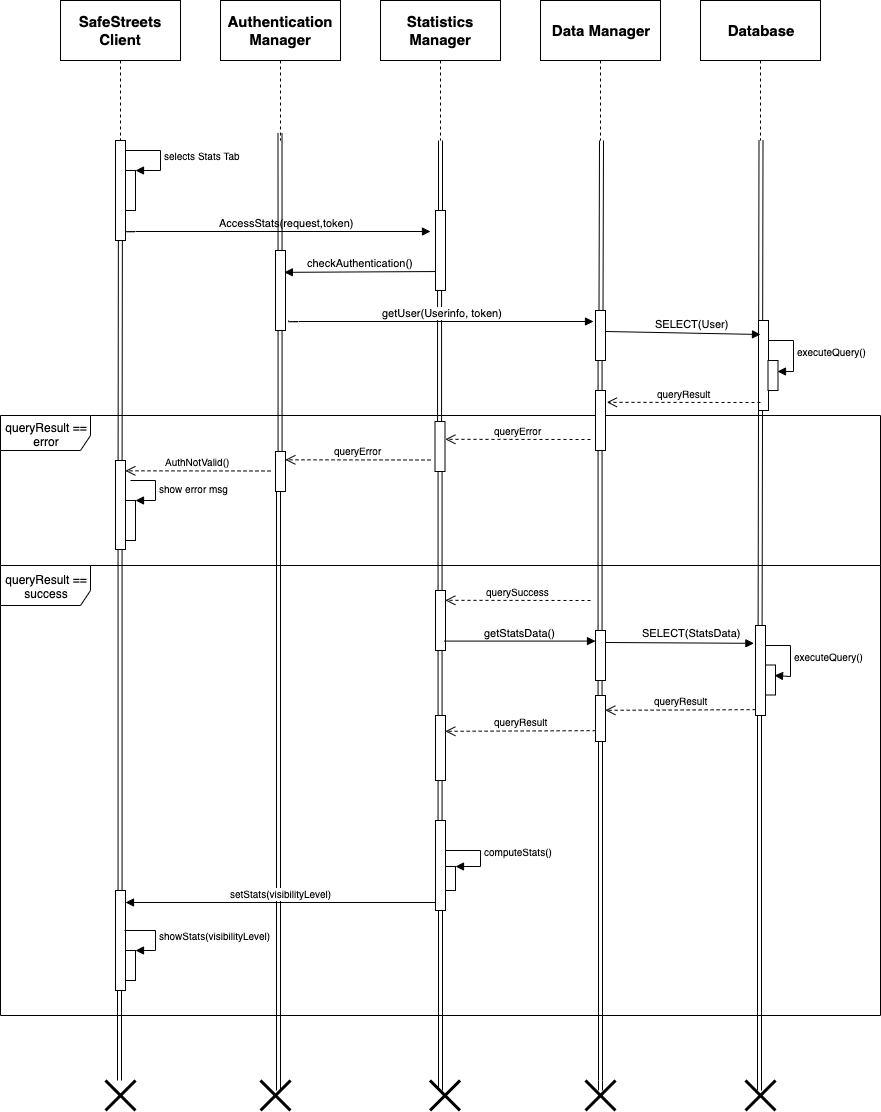
\includegraphics[scale=0.25]{Images/Diagrams/Runtime/stats_runtime.png}
			\caption{{\it SafeStreets} Statistics Access Runtime View}
	\end{figure}
	\pagebreak
	\noindent
	{\bf Tickets Validation Runtime View} \\
	The sixth sequence diagram \\
	\begin{figure}[H]
			\centering
			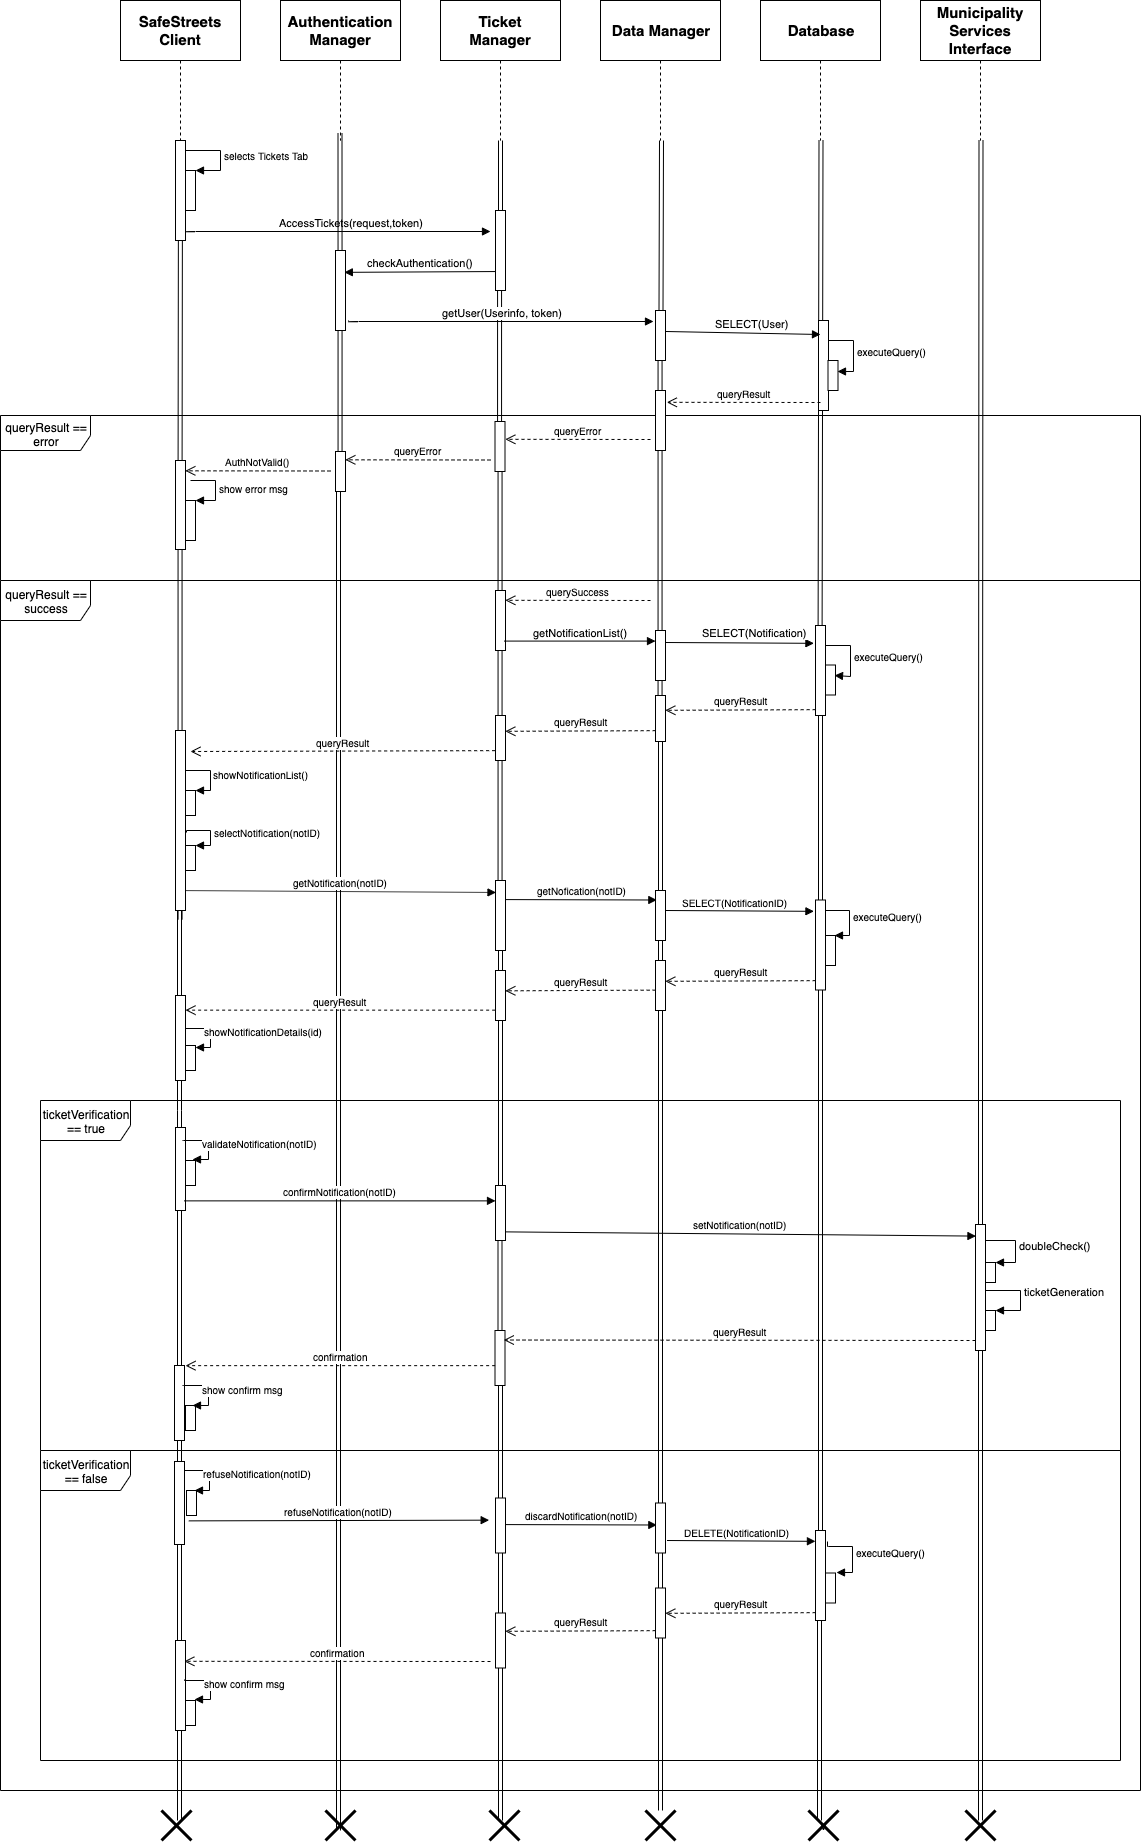
\includegraphics[scale=0.25]{Images/Diagrams/Runtime/tickets_runtime.png}
			\caption{{\it SafeStreets} Tickets Validation Runtime View}
	\end{figure}
	\pagebreak
	\noindent	
	{\bf Intervention Suggestion Runtime View} \\
	The seventh sequence diagram \\
	\begin{figure}[H]
			\centering
			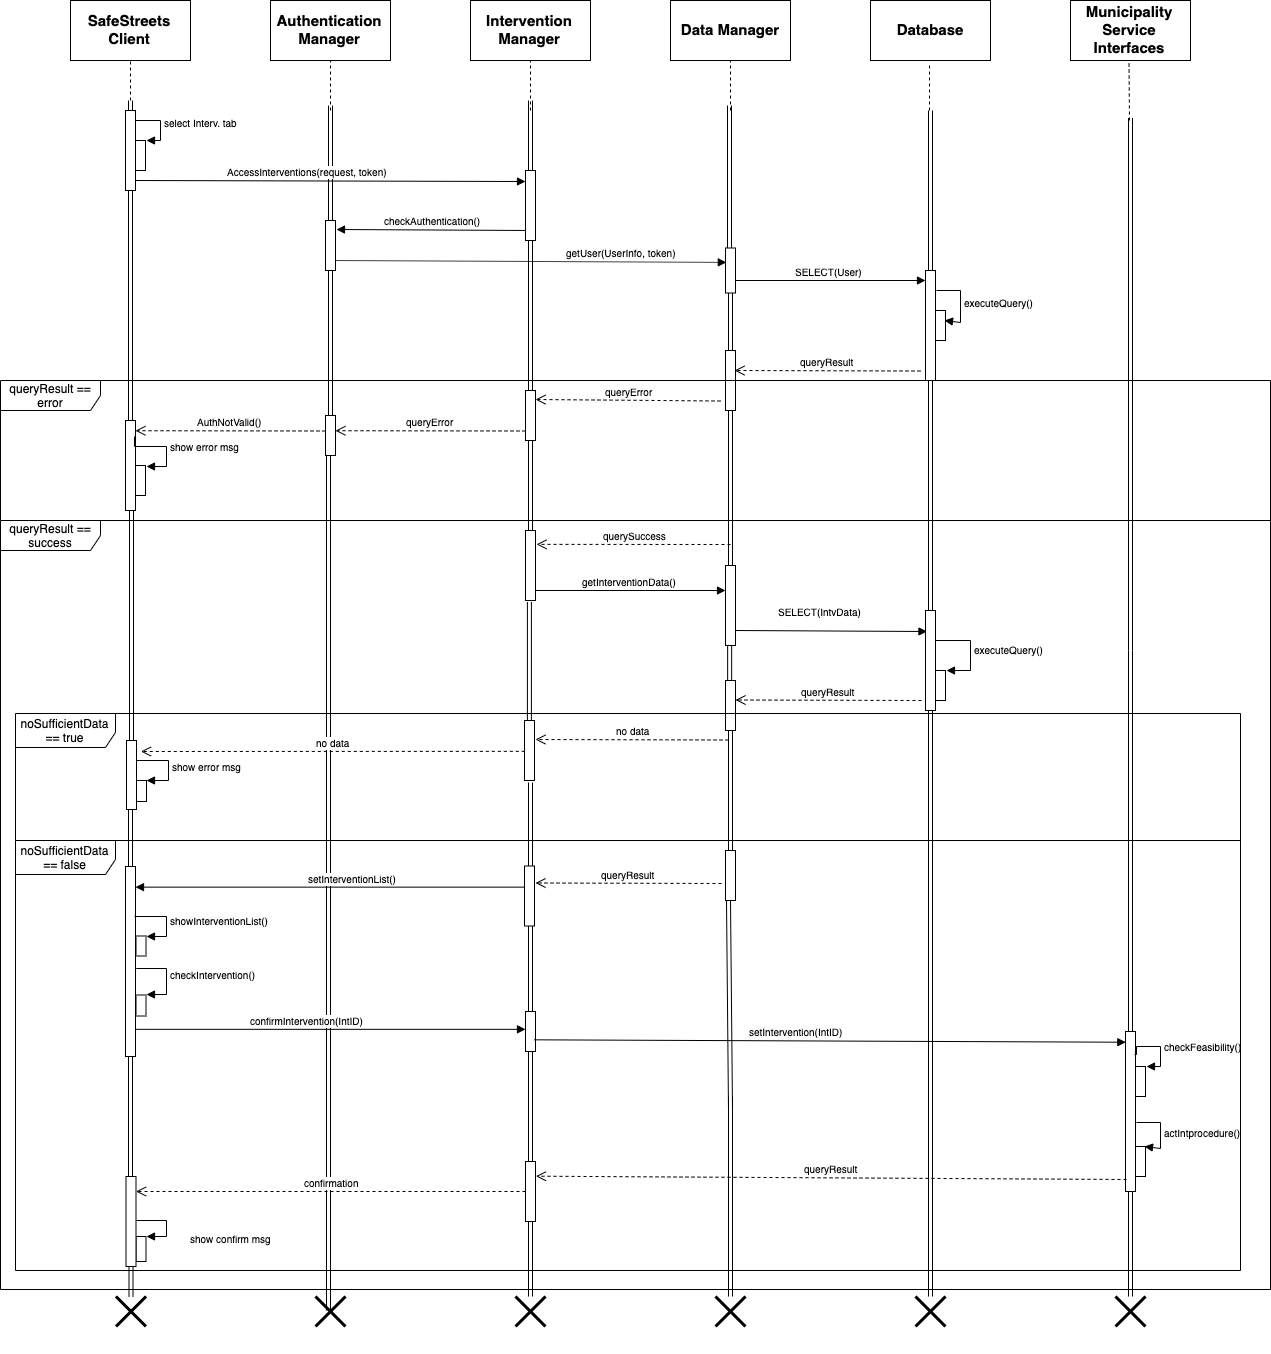
\includegraphics[scale=0.25]{Images/Diagrams/Runtime/interventions_runtime.png}
			\caption{{\it SafeStreets} Intervention Suggestion Runtime View}
	\end{figure}
	\pagebreak
	\noindent
	\subsection{Component Interfaces}
	{\bf Interface Diagram} \\
	The diagram below represents the Component View of the {\it System}, with methods that have been shown in the Runtime View. 
	\begin{comment}
		\begin{figure}[H]
			\centering
			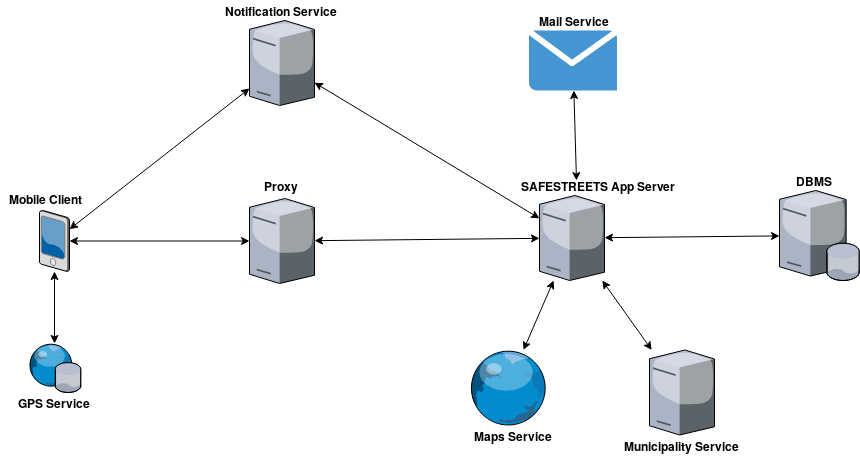
\includegraphics[scale=0.35]{Images/Diagrams/overview_diagram.png}
			\caption{Overview of the System}
		\end{figure}
	\end{comment}
	
	
	\subsection{Selected Architectural Styles and Patterns}
	{\bf Multi-tier Architecture} \\
	bla bla bla 
	\\ \\
	{\bf Thin Client} \\
	bla bla bla 
	\\ \\
	{\bf REST} \\
	bla bla 
	\\ \\ 
	{\bf MVC} \\
	bla bla bla
	\\ \\ 
	
	\subsection{Other Design Decisions}
	{\bf Database} \\
	bla bla 
	\\ \\ 
	{\bf Firewall} \\ 
	bla bla 
	\\ \\
	
\pagebreak

% User Interface Design - Section 3
\section{User Interface Design}
In the section 3.1 of the RASD document are explained in details all the User Interfaces and their design. So, for further information about the UI Design, refers to the RASD document. \\
In this section is provided an overview of the UX Application flow, using the UI mockups of the RASD. It's explained the flow of the application from the point of view of the {\it User} and from the point of view of the {\it Authorities}.
	\begin{figure}[H]
			\centering
			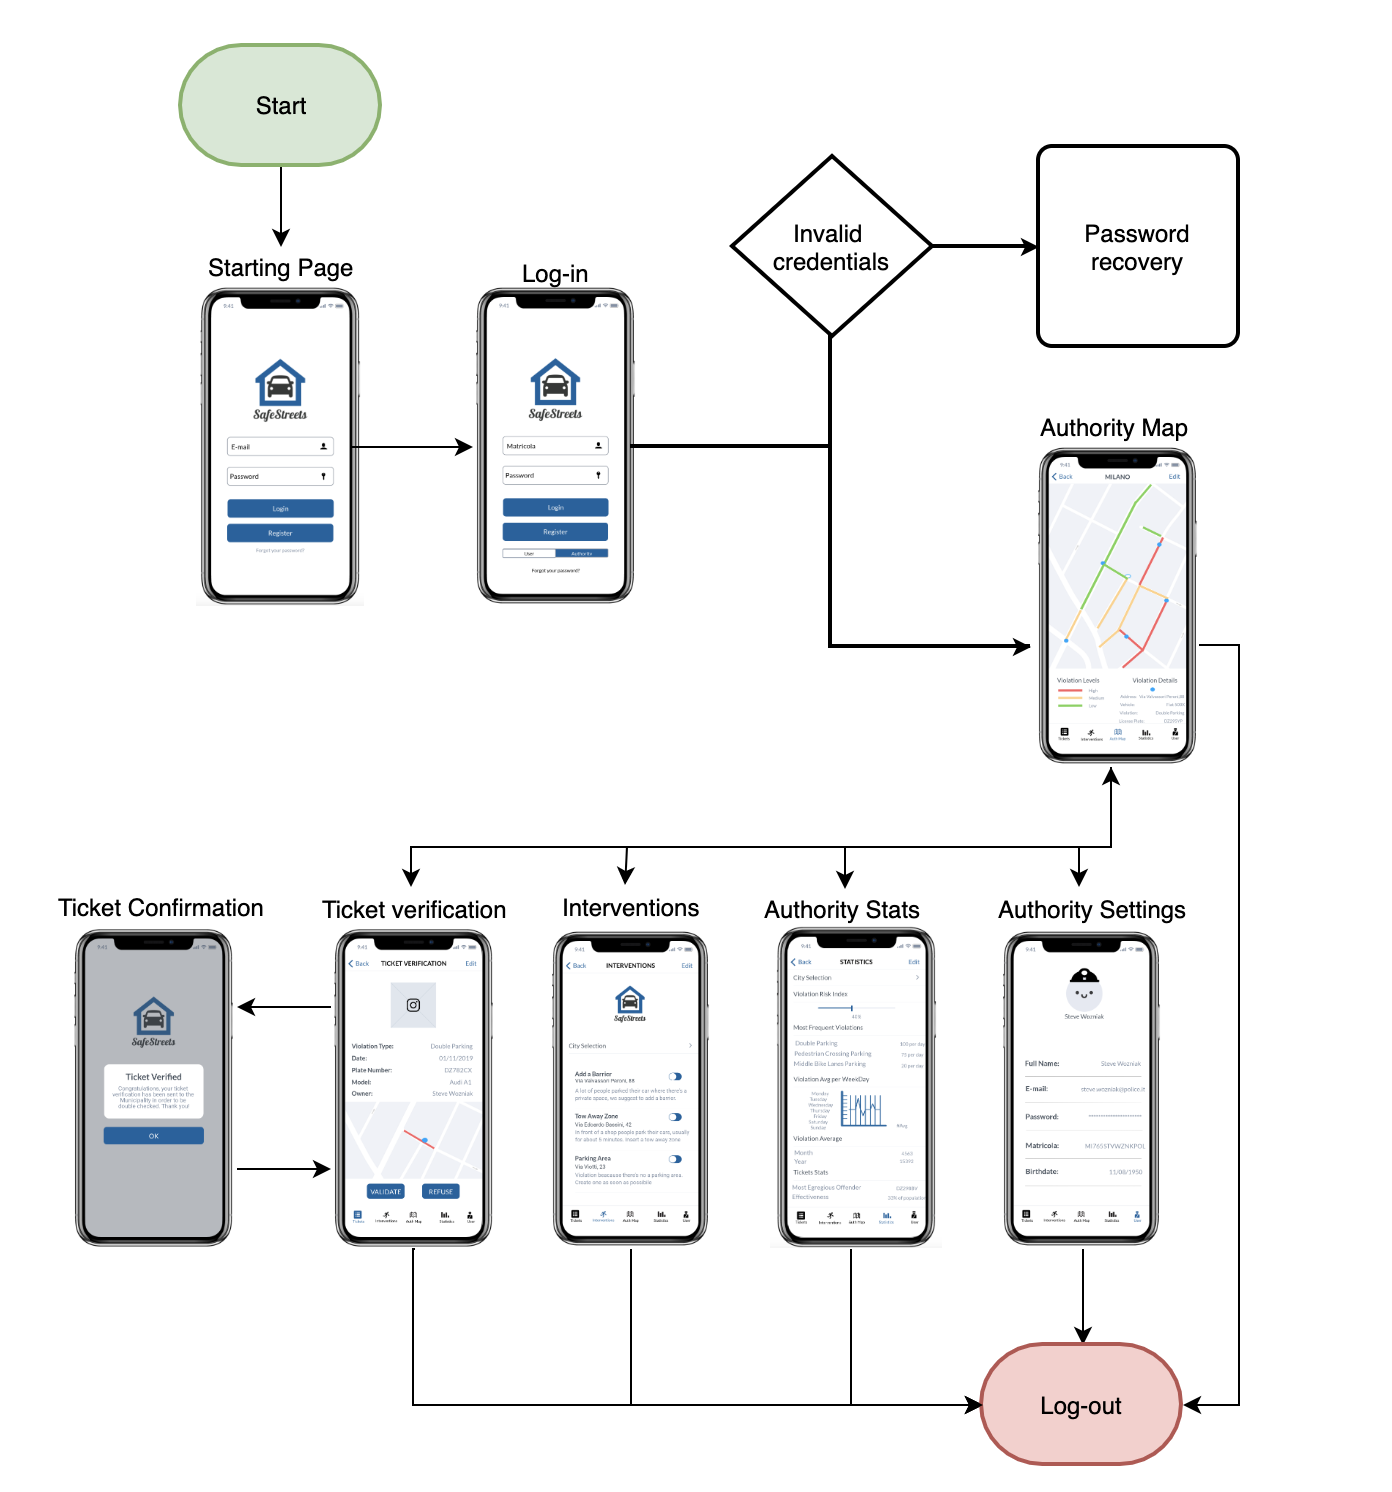
\includegraphics[scale=0.5]{Images/UX/user_ux_flow.png}
			\caption{{\it SafeStreets} User UX flow diagram}
	\end{figure}
	\begin{figure}[H]
			\centering
			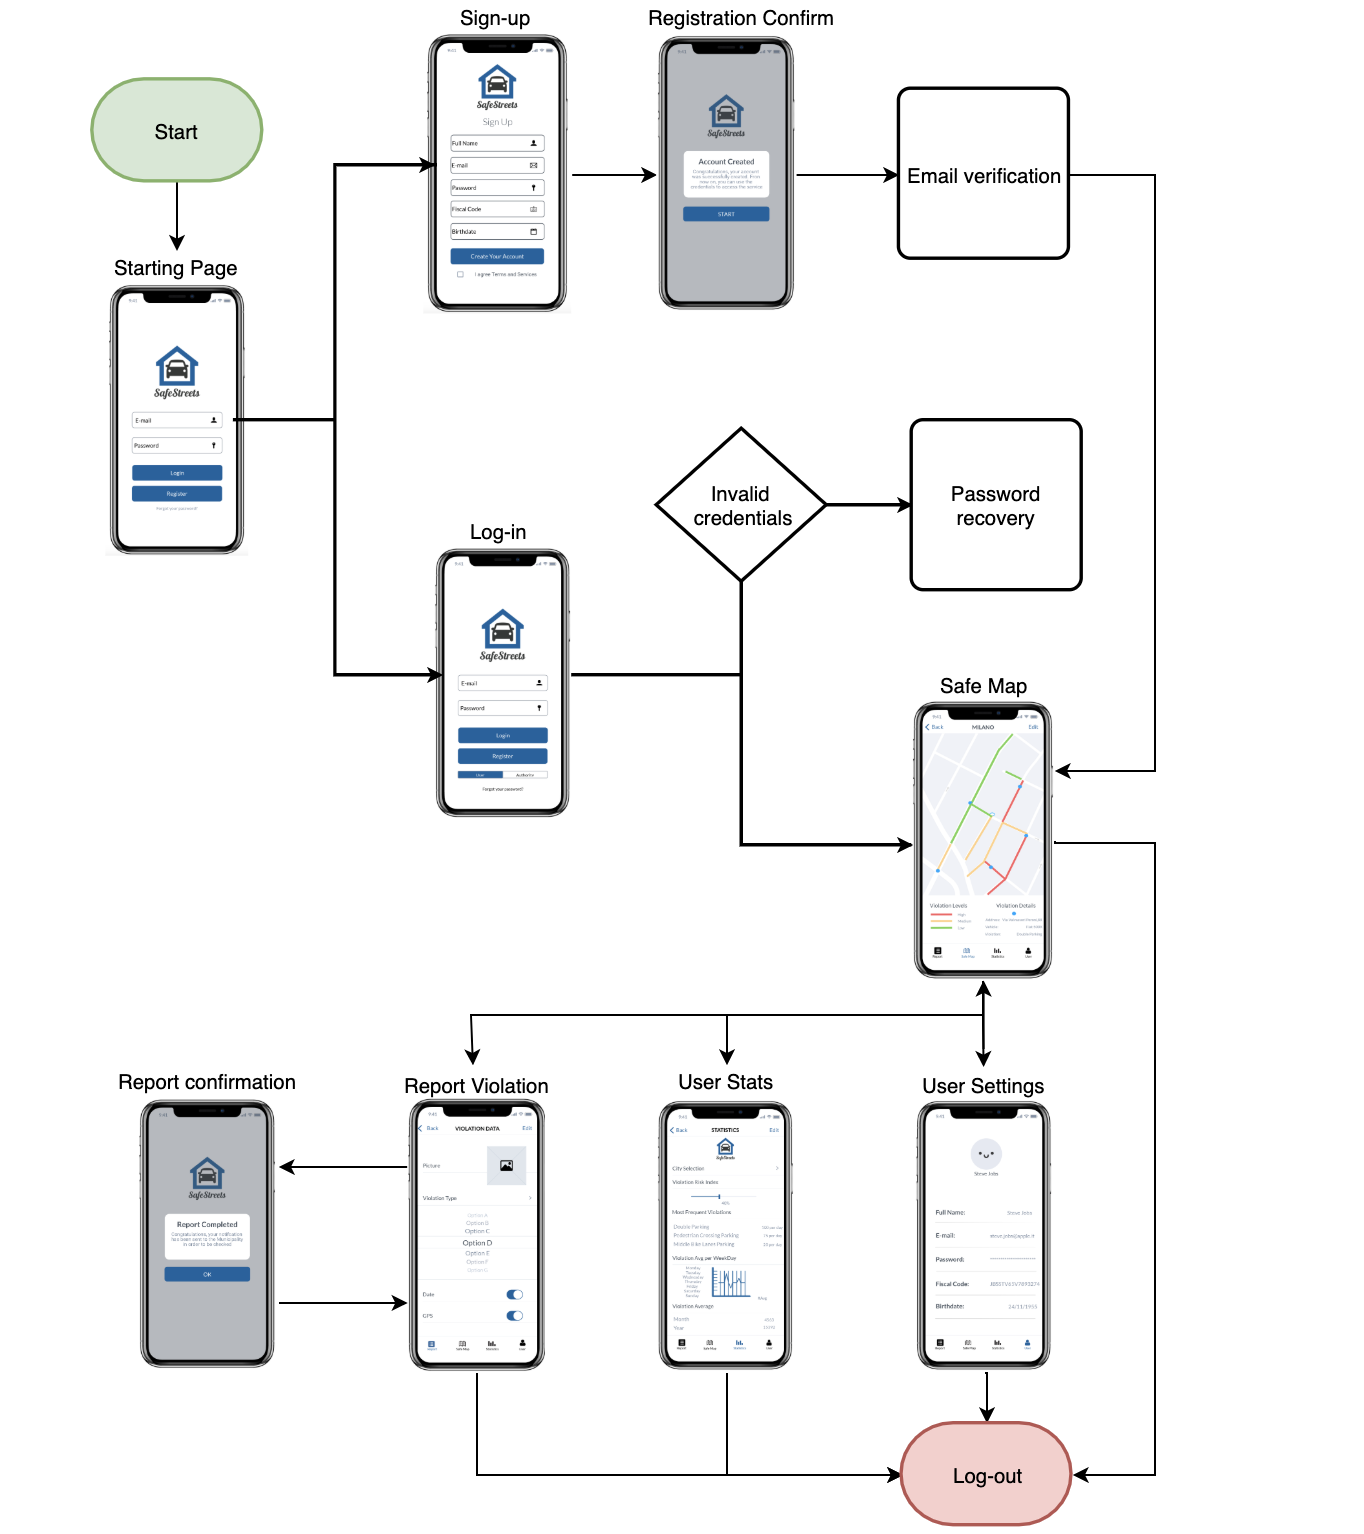
\includegraphics[scale=0.5]{Images/UX/authority_ux_flow.png}
			\caption{{\it SafeStreets} Authority UX flow diagram}
	\end{figure}

\pagebreak

% Requirements Traceability
\section{Requirements Traceability}
	
	\begin{longtable}{| p{5 cm} | p{8 cm} |} \hline
		Component (DD) & Requirements (RASD)  \\ \hline
		\newline Data Manager (Client) & 
		\begin{itemize}
			\item {[R13] Metadata, such as date and time, must be automatically re- trieved from the device.}
		\end{itemize}	\\ \hline
		\newline Authentication Manager & 
		\begin{itemize}
			\item  {[R1] The System allows account to be created as a simple User or Authority.}
			\item  {[R2] A User account can be created if the User provides the correct data: unique email and fiscal code.}
			\item  {[R4] Users and Authority can access the service if they log-in with their credentials.}
			\item  {[R5] The System must be able to check if the credentials are valid.
}
			\item  {[R9] Only User with an account can create and send a report.}
		\end{itemize}		\\	 \hline	
		\newline User Manager  & 
		\begin{itemize}
			\item  {[R6] The System must store all User credentials.}

		\end{itemize}		\\	 \hline	
		\newline Report Manager  & 
		\begin{itemize}
			\item  {[R8] The System gives a feedback to the User if the report process is done correctly.}
			\item  {[R9] Only User with an account can create and send a report.}
			\item  {[R10] The System must allow the User to take a picture of the violation.}
			\item  {[R12] The System must allow the User to select the violation type.}
			\item  {[R14] The System must allow the User to edit information before sending the report.}
		\end{itemize}		\\	 \hline	
		\newline Plate Image Controller & 
		\begin{itemize}
			\item  {[R7] The System must be able to analyse the picture and recognise
the plate number.
}
			\item  {[R8] The System gives a feedback to the User if the report process is done correctly.} 
			\item  {[R11] The System can accept or refuse the image loaded from the User.}
		\end{itemize}		\\	 \hline	
		\newline Statistics Manager & 
		\begin{itemize}
			\item  {[R18] The System must allow the User to visualise statistics derived from the data.}
			\item  {[R29] The System must allow the Authority to visualise statistics derived from tickets’ data.}
		\end{itemize}		\\	 \hline		
			\newline Ticket Manager & 
		\begin{itemize}
			\item  {[R23] The System must allow the Authority to access information
about the violation notification.}
			\item  {[R24] The System must allow the Authority to validate a ticket.}
			\item  {[R25] The System must allow the Authority to access sensible data
about the violation.}
			\item  {[R26] The System must advise the Authority that the violation de- tails process is done correctly.}
		\end{itemize}		\\	 \hline	
			\newline Intervention Manager & 
		\begin{itemize}
			\item  {[R20] The System must be able to identify viability issues based on data.}
			\item  {[R21] The System must suggest solution to address viability issue.}
			\item  {[R22] The System must allow the Authority to access the list of possible interventions.
}
			\item  {[R23B] The System must allow the Authority to establish if the inter- vention is feasible solutions or not.}
		\end{itemize}		\\	 \hline	
			\newline Data Manager & 
		\begin{itemize}
			\item {[R6] The System must store all User credentials.}

			\item  {[R15] The System must be able to store all the notifications’ data.}
			\item   {[R27] The System must be able to store all the tickets’ data.}
		\end{itemize}		\\	 \hline			
		\caption{Requirements Traceability}	
		
	\end{longtable}
	
	\pagebreak
	
	
% Testing - Section 5
\section{Implementation, Integration and Test Plan}
	\subsection{Overview}
	The {\it System} is divided in many components, that can be divided in the following sub-systems:
	\begin{itemize}
		\item Frontend Components: this is Client application subsystem, containing the presentation and the data manager components.
		\item Back-end Components: this is the Business Logic subsystem with all its components that interacts with the database. 
		\item External Components: this are the external components that interacts with the {\it System}, such as the Map and GPS services.  
	\end{itemize}
	The strategy used to design the {\it System} was {\it Top-Down}, defining the sub-systems described above at a high-level, then refining and detailing them with all the details needed.\\
	The implementation and testing approach will follow a combination of both {\it Top-Down} and {\it Bottom-Up} strategies because it's the most reasonable choice for relatively small components and sub-systems. \\ 
	In the following paragraphs it will be presented the order of the implementation and of the integration testing between components.
		
	\subsection{Implementation}
	The implementation of the different components will be parallelised in order to divide the work between developers and for speeding up the implementation process. \\
	The order of the implementation is:
	\begin{itemize}
		\item Implementation of the Database component
		\item Implementation of Business Logic and Client components
		\item Integration of component with external service interfaces 
	\end{itemize}
	The implementation of the Database consist of instance creation on an external  platform provider and the creation of tables and schemes. 
	The implementation of the Back-end Components is parallelised, so the Business Logic (Server) and Client will be developed by different developers and then linked together. 
	The integration with external services consists of a series of API calls to the external services that are already implemented. \\ \\ \\ \\ \\ \\ \\ \\
	The Business Logic implementation will follow this order. If there are some components on the same line means that they will be implemented in parallel:
	\begin{enumerate}
		\item Data Manager
		\item Authentication Manager, User Manager
		\item Report Manager, Plate Img Controller
		\item Statistics, Ticket, Intervention Manager
	\end{enumerate}
	The Client implementation will follow this order:
	\begin{enumerate}
		\item Data Manager
		\item Presentation
	\end{enumerate}
	The Data Manager is critical because it represents to unique point of access to the Database and it is the component that interacts with all the components that compute the application logic and operate on the basis of the Data Manager retrieval capacity.
	\subsection{Integration and Testing}
	\pagebreak
		
% Effort - Section 6
\section{Effort Spent}
\begin{longtable}{| p{2 cm} | p{6 cm} | p{1 cm} |} 
			\hline
			{\bf Date} & {\bf Task} & {\bf Hours}\\
			\hline
			XX/XX/XX & XX & X \\
			\hline
			& & {\bf Total} \\
			\hline
			& & XX \\
			\hline
			\caption{Adriano Mundo's effort} 
\end{longtable}

\begin{longtable}{| p{2 cm} | p{6 cm} | p{1 cm} |} 
			\hline
			{\bf Date} & {\bf Task} & {\bf Hours}\\
			\hline
			XX/XX/XX & XX & X \\
			\hline
			& & {\bf Total} \\
			\hline
			& & XX \\
			\hline
			\caption{Francesco Rota's effort} 
\end{longtable}

\begin{longtable}{| p{2 cm} | p{6 cm} | p{1 cm} |} 
			\hline
			{\bf Date} & {\bf Task} & {\bf Hours}\\
			\hline
			XX/XX/XX & XX & X \\
			\hline
			& & {\bf Total} \\
			\hline
			& & XX \\
			\hline
			\caption{Salvatore Fadda's effort} 
\end{longtable}
	
	
\end{document}
